% =============================================================================
% INFORME — Evaluación 3 ECSD · Caso 2: Línea de Producción con Balanceo Dinámico
% BORRADOR generado desde las bitácoras de docs/fases/ — revisar antes de entregar.
% Compilar con pdfLaTeX o LuaLaTeX (misma plantilla del informe anterior).
% =============================================================================
\documentclass[12pt,a4paper]{article}

\usepackage[spanish, es-tabla]{babel}
\deactivatequoting
\usepackage[margin=2.54cm, top=4.2cm, bottom=3.2cm]{geometry}
\usepackage{graphicx}
\usepackage{multirow}
\usepackage{hyperref}
\usepackage{amsmath}
\usepackage{amssymb}
\usepackage{array}
\usepackage{booktabs}
\usepackage{xcolor}
\usepackage{fancyhdr}
\usepackage{titlesec}
\usepackage{enumitem}
\usepackage{parskip}
\usepackage{caption}
\usepackage{float}
\usepackage{eso-pic}
\usepackage{setspace}
\usepackage{listings}
\usepackage{tikz}
\usetikzlibrary{shapes.geometric, arrows, positioning, calc}

\usepackage{iftex}
\ifpdftex
  \usepackage[utf8]{inputenc}
  \usepackage[T1]{fontenc}
  \usepackage{lmodern}
  \providecommand{\robotocon}{\sffamily}
\else
  \usepackage{fontspec}
  \IfFontExistsTF{Libre Franklin}
    {\setmainfont{Libre Franklin}[UprightFont = *-Thin, BoldFont = *-Bold]}
    {\IfFontExistsTF{Segoe UI}{\setmainfont{Segoe UI}}{}}
  \IfFontExistsTF{Roboto Condensed}
    {\newfontfamily\robotocon{Roboto Condensed}[UprightFont = *-Regular, BoldFont = *-Bold]}
    {\IfFontExistsTF{Bahnschrift}{\newfontfamily\robotocon{Bahnschrift}}{\providecommand{\robotocon}{\sffamily}}}
\fi

\definecolor{usachteal}{RGB}{0,155,138}
\definecolor{usachdark}{RGB}{28,32,38}
\definecolor{backcolour}{rgb}{0.96,0.96,0.96}
\hypersetup{hidelinks, colorlinks=true, linkcolor=usachdark, citecolor=usachteal, urlcolor=usachteal}

\lstdefinestyle{codigo}{
    backgroundcolor=\color{backcolour},
    basicstyle=\ttfamily\footnotesize,
    breaklines=true,
    captionpos=b,
    keepspaces=true,
    showstringspaces=false,
    tabsize=2
}
\lstset{style=codigo}

\tikzset{
  etapa/.style={rectangle, rounded corners, minimum width=2.3cm, minimum height=0.9cm, text centered, draw=usachdark, fill=usachdark!5, font=\small},
  etaparep/.style={rectangle, rounded corners, minimum width=2.3cm, minimum height=0.9cm, text centered, draw=usachteal, fill=usachteal!15, font=\small\bfseries},
  colaq/.style={rectangle, minimum width=1.1cm, minimum height=0.7cm, text centered, draw=usachdark!60, fill=orange!10, font=\scriptsize},
  nodo/.style={rectangle, rounded corners, draw=usachteal, fill=usachteal!8, font=\small\bfseries, inner sep=8pt},
  arrow/.style={thick,->,>=stealth,color=usachdark}
}

\AddToShipoutPictureBG{%
  \AtPageUpperLeft{%
    \raisebox{-\paperheight}{%
      
\includegraphics[width=\paperwidth, height=\paperheight]{portada.png}%
    }%
  }%
}

\titleformat{\section}{\large\bfseries\color{usachteal}}{\thesection.}{0.5em}{}
\titleformat{\subsection}{\normalsize\bfseries\color{usachdark}}{\thesubsection.}{0.5em}{}
\titleformat{\subsubsection}{\small\bfseries\color{usachteal}}{\thesubsubsection.}{0.5em}{}
\titlespacing*{\section}{0pt}{14pt}{6pt}
\titlespacing*{\subsection}{0pt}{10pt}{4pt}
\titlespacing*{\subsubsection}{0pt}{8pt}{2pt}

\pagestyle{fancy}
\fancyhf{}
\setlength{\headheight}{52pt}
\fancyhead[L]{{\small\robotocon\bfseries\color{usachdark} USACH\;|\;\color{usachteal} EVALUACIÓN 3 ECSD — CASO 2}}
\fancyhead[R]{\small\color{gray}\thepage}
\renewcommand{\headrulewidth}{0pt}
\renewcommand{\footrulewidth}{0pt}

\setstretch{1.25}
\setlength{\parskip}{6pt}
\setlength{\parindent}{0pt}
\tolerance=1
\emergencystretch=\maxdimen
\hyphenpenalty=10000
\hbadness=10000

\newcolumntype{C}[1]{>{\centering\arraybackslash}p{#1}}
\newcolumntype{L}[1]{>{\raggedright\arraybackslash}p{#1}}

\author{César Olivares \\ Simón García-Huidobro}

\begin{document}

% ============================== PORTADA ======================================
\begin{titlepage}
\begin{flushright}
\begin{tabular}{cl}
 & \multirow{4}{*}{
\includegraphics[width=2.8cm]{logoBN.png}} \\[5pt]
 \textbf{UNIVERSIDAD DE SANTIAGO DE CHILE} & \\[3pt]
 \textbf{DEPARTAMENTO DE INGENIERÍA MECÁNICA} & \\[3pt]
 \textbf{INGENIERÍA CIVIL MECATRÓNICA} &
\end{tabular}
\end{flushright}

\vspace{1.5cm}
\begin{center}
{\Large \textbf{Estructura de Computadores y Sistemas Distribuidos}}\\[8pt]
{\large \textbf{Evaluación 3 — Caso 2: Línea de Producción con Balanceo Dinámico}}\\[12pt]
{\small \textbf{Sistema distribuido de simulación de una línea conservera con coordinación por colas, detección de cuellos de botella en vivo y tablero de operaciones}}
\end{center}

\vspace{1.5cm}
\begin{center}
\textbf{Integrantes:}\\[4pt]
César Olivares\\
Simón García-Huidobro\\[12pt]
\textbf{Profesor:}\\[4pt]
Daniel Calderón R.
\end{center}
\vfill
\begin{center}
\textbf{Santiago, Chile\\ \today}
\end{center}
\end{titlepage}

\tableofcontents
\newpage

% =============================================================================
\section{Introducción}

Este informe presenta el diseño, implementación y evaluación experimental de un
sistema distribuido que simula una \textbf{línea de producción con balanceo
dinámico de carga} (Caso 2). El dominio elegido es una planta conservera
\textbf{ficticia} de jurel en lata de 425~g, inspirada en la industria
conservera nacional, con cuatro etapas en serie separadas por \textbf{colas de
trabajo}: cada cola es, literalmente, la fila de lotes que esperan frente a la
etapa siguiente. Si una etapa procesa más lento de lo que le llega trabajo, su
fila crece — y esa fila creciente es exactamente lo que este sistema mide y
diagnostica en vivo.

\begin{figure}[H]
\centering
\begin{tikzpicture}[node distance=0.35cm,
  etapac/.style={rectangle, rounded corners, minimum width=2.15cm, minimum height=1.05cm,
                 text centered, draw=usachdark, fill=usachdark!5, font=\scriptsize, align=center},
  etaparc/.style={rectangle, rounded corners, minimum width=2.15cm, minimum height=1.05cm,
                  text centered, draw=usachteal, fill=usachteal!15, font=\scriptsize\bfseries, align=center}]
  \node (q1) [colaq] {cola};
  \node (e1) [etapac, right=of q1] {\textbf{Fileteado}\\ ciclo 4 s};
  \node (q2) [colaq, right=of e1] {cola};
  \node (e2) [etaparc, right=of q2] {Envasado\\ ciclo 12 s\\ $\times$1--3 réplicas};
  \node (q3) [colaq, right=of e2] {cola};
  \node (e3) [etapac, right=of q3] {\textbf{Sellado}\\ ciclo 3 s};
  \node (q4) [colaq, right=of e3] {cola};
  \node (e4) [etapac, right=of q4] {\textbf{Esterilización}\\ ciclo 7 s};
  \node (fin) [right=0.45cm of e4, font=\scriptsize\bfseries, text=usachteal] {listos};
  \draw [arrow] (q1) -- (e1); \draw [arrow] (e1) -- (q2);
  \draw [arrow] (q2) -- (e2); \draw [arrow] (e2) -- (q3);
  \draw [arrow] (q3) -- (e3); \draw [arrow] (e3) -- (q4);
  \draw [arrow] (q4) -- (e4); \draw [arrow] (e4) -- (fin);
  \node [above=0.12cm of q1, font=\tiny, text=usachdark!70] {órdenes};
\end{tikzpicture}
\caption{La línea de producción: cuatro etapas en serie unidas por colas de
trabajo. Envasado, la etapa más lenta, es la replicada.}
\label{fig:pipeline}
\end{figure}

\begin{table}[H]
\centering
\caption{Etapas de la línea y tiempos de ciclo simulados (supuesto declarado, §\ref{sec:supuestos}).}
\small
\begin{tabular}{L{3cm} L{4.5cm} C{2.5cm} C{2.5cm}}
\toprule
\textbf{Etapa} & \textbf{Naturaleza} & \textbf{Ciclo (s/lote)} & \textbf{Réplicas} \\
\midrule
Fileteado & Manual, paralelizable & 4 & 1 \\
\textbf{Envasado} & Máquina continua & \textbf{12} & \textbf{1--3 (replicada)} \\
Sellado & Máquina rápida & 3 & 1 \\
Esterilización & Autoclave, ciclo fijo & 7 & 1 \\
\bottomrule
\end{tabular}
\end{table}

La unidad de trabajo es el \textbf{lote} (una cantidad de latas del mismo
formato). El sistema cumple los requisitos del enunciado: arquitectura
distribuida con más de tres servicios en tres nodos lógicos, una etapa
replicada detrás de un mecanismo de balanceo, coordinación del reparto sin
condiciones de carrera, detección de cuellos de botella \emph{en vivo},
persistencia, interfaz de operación con interacción real, y despliegue completo
con un solo comando (\texttt{docker compose up}).

El resultado experimental central (§\ref{sec:experimentos}) demuestra
literalmente la premisa del caso: al escalar envasado de 1 a 2 réplicas, el
cuello de botella \textbf{se desplaza} de envasado a esterilización y el lead
time cae un 21~\%; una tercera réplica ya casi no mejora nada, porque el límite
se mudó de etapa.

% =============================================================================
\section{Arquitectura del sistema}

\subsection{Servicios}

\begin{table}[H]
\centering
\caption{Servicios del sistema. Todos en Python; API con FastAPI, UI con Streamlit.}
\small
\begin{tabular}{L{3.2cm} L{6.8cm} L{3.6cm}}
\toprule
\textbf{Servicio} & \textbf{Responsabilidad} & \textbf{Tecnología} \\
\midrule
\texttt{orders-api} & Crea órdenes, las persiste y las encola & FastAPI + SQLite + Redis \\
\texttt{estacion} ($\times$4--6) & Procesa lotes; una imagen única configurada por variables de entorno & Python + Redis + SQLite \\
\texttt{metrics-api} & Calcula espera, servicio y lead time; detecta el cuello de botella & FastAPI + SQLite + Redis \\
\texttt{ui} & Tablero de operaciones: timeline, carga por réplica, alertas, histórico, creación de órdenes & Streamlit \\
Redis & Colas de trabajo y estado de réplicas & Redis 7 \\
\bottomrule
\end{tabular}
\end{table}

Las cuatro estaciones son \textbf{un solo programa} desplegado cuatro (o más)
veces: la etapa, sus colas de entrada/salida y su tiempo de ciclo llegan por
variables de entorno (\texttt{NOMBRE\_ETAPA}, \texttt{COLA\_ENTRADA},
\texttt{COLA\_SALIDA}, \texttt{TIEMPO\_CICLO}). Escalar la etapa replicada es
\texttt{docker compose up --scale envasado=3}: ninguna réplica sabe cuántas
hermanas tiene ni necesita saberlo.

\subsection{Nodos lógicos y su justificación}
\label{sec:nodos}

\begin{figure}[H]
\centering
\begin{tikzpicture}[node distance=0.6cm and 1.2cm]
  \node (na) [nodo, minimum width=3.6cm, minimum height=2.6cm, label={[font=\small\bfseries]above:NODO A — operación}] {};
  \node at (na.center) [align=center, font=\small] {Streamlit (UI)\\ orders-api};
  \node (nb) [nodo, right=of na, minimum width=4.2cm, minimum height=2.6cm, label={[font=\small\bfseries]above:NODO B — procesamiento}] {};
  \node at (nb.center) [align=center, font=\small] {fileteado\\ envasado $\times$1--3\\ sellado · esterilización};
  \node (nc) [nodo, right=of nb, minimum width=3.6cm, minimum height=2.6cm, label={[font=\small\bfseries]above:NODO C — estado}] {};
  \node at (nc.center) [align=center, font=\small] {Redis\\ metrics-api\\ SQLite};
  \draw [arrow, <->] (na) -- (nb);
  \draw [arrow, <->] (nb) -- (nc);
  \draw [arrow, <->] (na.south) to[bend right=18] (nc.south);
\end{tikzpicture}
\caption{Los tres nodos lógicos y sus comunicaciones (HTTP/JSON y protocolo Redis).}
\end{figure}

La agrupación no es arbitraria: cada nodo reúne responsabilidades que
\textbf{cambian de escala por motivos distintos}, el criterio clásico para
particionar un sistema distribuido \cite{tanenbaum}. El nodo B es el único que se
replica bajo carga (agregar capacidad de procesamiento = agregar contenedores
ahí). El nodo C concentra el estado compartido, que por ser compartido
\emph{no puede} duplicarse sin coordinación adicional. El nodo A expone el
sistema al operador y escala con los usuarios, no con la producción.

\textbf{Por qué mantener dos o más nodos} (exigencia de la rúbrica): además de
ser requisito del enunciado, separa dominios de falla y de recursos — la
saturación de CPU de las estaciones (nodo B) no degrada la atención HTTP del
operador (nodo A) ni la integridad del estado (nodo C); y permite dimensionar
hardware distinto para cargas distintas (B necesita CPU, C necesita disco
confiable). La sección §\ref{sec:resiliencia} discute cómo se abordaría la
resiliencia sobre esta misma división.

\subsection{Flujo de una orden}

Una orden nace en \texttt{orders-api} (\texttt{POST /ordenes}): se inserta en
SQLite, se registra su evento \texttt{entra\_cola} y su id se empuja a
\texttt{cola:fileteado} — todo dentro de una transacción, de modo que si Redis
no responde no quedan ``órdenes fantasma'' guardadas pero nunca encoladas.
Cada estación repite el mismo ciclo: reclama un id de su cola de entrada
(\texttt{BRPOP}), registra \texttt{inicia}, simula el ciclo
(\texttt{sleep(TIEMPO\_CICLO)}), registra \texttt{termina} y
\texttt{entra\_cola} de la etapa siguiente, y empuja el id a la cola siguiente.
La última etapa marca la orden como \texttt{terminada}.

% =============================================================================
\section{Decisiones de diseño}

\subsection{Balanceo por demanda: cola \emph{pull}, no balanceador clásico}
\label{sec:pull}

El enunciado sugiere ``réplicas detrás de un balanceador''. Decidimos —y es una
\textbf{decisión nuestra que defendemos aquí}— implementar el balanceo como
\textbf{cola de trabajo compartida}: las réplicas \emph{piden} un lote cuando
quedan libres, en vez de recibirlo asignado por una pieza intermedia — el
patrón de consumidores en competencia sobre un broker de mensajes
\cite{kleppmann}.

\begin{enumerate}[leftmargin=*]
  \item Es lo único que produce balanceo \textbf{dinámico} real. Un
        round-robin le seguiría enviando lotes a una réplica lenta o atascada;
        con reparto por demanda, la réplica lenta simplemente pide menos veces.
        El experimento 4 (§\ref{sec:exp4}) lo muestra con datos: 11/12/7.
  \item Resuelve la condición de carrera \textbf{con el mismo mecanismo}: la
        extracción atómica de la cola es a la vez el reparto y la garantía de
        exclusión (§\ref{sec:carrera}), sin una pieza extra que configurar ni
        un lock con expiración que se pueda vencer en el momento equivocado.
  \item El reparto emergente es proporcional a la capacidad real de cada
        réplica, sin conocer cuántas hay: \texttt{--scale envasado=3} funciona
        sin tocar configuración.
\end{enumerate}

El ``balanceador'' del enunciado existe, pero es la cola: el punto único por
el que pasa el trabajo y que decide quién procesa qué. Si se exigiera un
balanceador HTTP clásico, un Nginx delante de las réplicas cubriría las
consultas de estado; para el \emph{trabajo}, el reparto por demanda es
estrictamente superior en este caso.

\subsection{Coordinación y condición de carrera: provocarla antes de resolverla}
\label{sec:carrera}

El requisito de coordinación (``que dos réplicas no tomen la misma orden'') se
abordó en dos pasos deliberados, ambos preservados en el historial de commits:

\textbf{Versión ingenua (commiteada rota a propósito).} Reclamar una orden en
dos operaciones: mirar la cola (\texttt{LRANGE}) y después sacar el elemento
(\texttt{LREM}). Entre ambas hay una ventana en la que otra réplica ve
\emph{la misma} orden. Con 3 réplicas y 200 órdenes, el experimento reprodujo
órdenes procesadas dos veces — la evidencia de que el problema es real y no
teórico.

\textbf{Versión atómica.} \texttt{BRPOP}: extracción bloqueante en \textbf{una
sola operación indivisible} \cite{redis}. Redis, al ser monohilo en la atención
de comandos, garantiza que cada elemento se entrega a exactamente una réplica
aunque haya varias esperando sobre la misma cola. Mismo experimento:
\textbf{0 duplicados en 200 órdenes}.

\begin{figure}[H]
\centering
\begin{tikzpicture}[
  rep/.style={rectangle, rounded corners, draw=usachdark, fill=usachdark!5, font=\scriptsize, minimum width=1.7cm, minimum height=0.55cm},
  msg/.style={font=\tiny, midway, above, sloped},
  cola/.style={rectangle, draw=usachdark!60, fill=orange!10, font=\scriptsize\bfseries, minimum width=1.9cm, minimum height=0.55cm},
  mal/.style={font=\scriptsize\bfseries, text=red!70!black},
  bien/.style={font=\scriptsize\bfseries, text=usachteal}]
  % Panel izquierdo: ingenua
  \node (tit1) [font=\scriptsize\bfseries, text=usachdark] at (0,2.1) {Versión ingenua: mirar y sacar (2 pasos)};
  \node (colaA) [cola] at (0,1.3) {cola: lote \#42};
  \node (r1a) [rep] at (-1.6,-0.2) {réplica 1};
  \node (r2a) [rep] at (1.6,-0.2) {réplica 2};
  \draw [arrow] (colaA.south west) -- (r1a.north) node[msg] {ve \#42};
  \draw [arrow] (colaA.south east) -- (r2a.north) node[msg] {ve \#42};
  \node (dup) [mal] at (0,-1.05) {ambas procesan \#42: duplicado};
  % Panel derecho: atómica
  \node (tit2) [font=\scriptsize\bfseries, text=usachdark] at (7.6,2.1) {Versión atómica: \texttt{BRPOP} (1 paso)};
  \node (colaB) [cola] at (7.6,1.3) {cola: \#42, \#43};
  \node (r1b) [rep] at (6.0,-0.2) {réplica 1};
  \node (r2b) [rep] at (9.2,-0.2) {réplica 2};
  \draw [arrow] (colaB.south west) -- (r1b.north) node[msg] {recibe \#42};
  \draw [arrow] (colaB.south east) -- (r2b.north) node[msg] {recibe \#43};
  \node (ok) [bien] at (7.6,-1.05) {cada lote a exactamente una réplica};
\end{tikzpicture}
\caption{La condición de carrera y su solución. A la izquierda, entre
``mirar'' y ``sacar'' hay una ventana en la que dos réplicas ven el mismo
lote; a la derecha, la extracción es una única operación indivisible y la
ventana no existe.}
\label{fig:carrera}
\end{figure}

Se prefirió la operación atómica de cola por sobre un lock/contador distribuido
(la alternativa que el enunciado menciona como ejemplo) porque elimina la
ventana en vez de administrarla: no hay TTL que expire a mitad de un ciclo ni
liberación de lock que se pueda olvidar. El requisito del ``lock/contador
distribuido'' está cubierto por el mismo Redis que serializa las extracciones.

\subsection{Criterio de cuello de botella: espera, no servicio}
\label{sec:criterio}

El enunciado no define qué es un cuello de botella; el criterio es una
\textbf{decisión nuestra} y es el argumento técnico central del proyecto:

\begin{quote}
El cuello de botella es la etapa con \textbf{mayor tiempo de espera promedio en
una ventana móvil}, siempre que supere su umbral de advertencia. Si ninguna lo
supera, no hay cuello (\texttt{cuello: null}).
\end{quote}

Con los eventos de cada orden se definen, por etapa:
\[
\text{espera} = t_{\text{inicia}} - t_{\text{entra\_cola}}, \qquad
\text{servicio} = t_{\text{termina}} - t_{\text{inicia}}, \qquad
\text{lead time} = t_{\text{fin}} - t_{\text{creada}}
\]

Un tiempo de \emph{servicio} alto solo dice que la tarea es larga; el atasco es
trabajo llegando más rápido de lo que la etapa lo drena, y eso se manifiesta en
la \emph{espera} — la misma relación entre llegadas, capacidad y fila que
formaliza la ley de Little \cite{little} y que la teoría de las restricciones
usa para localizar la limitante de un proceso \cite{goldratt}. La analogía
cotidiana: en un supermercado, que un cajero sea lento no significa que haya
atasco; el atasco es la \emph{fila} que crece frente a su caja. El experimento
2 lo ilustra con datos (Figura \ref{fig:espera_vs_servicio}): la etapa señalada
como cuello (esterilización, ciclo 7~s) tiene un ciclo \textbf{más corto} que
envasado (12~s) — un criterio por tiempo de servicio jamás la habría
encontrado.

\begin{figure}[H]
\centering
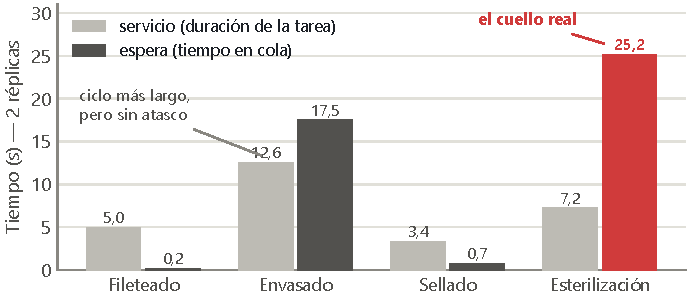
\includegraphics[width=0.82\textwidth]{figuras/fig_espera_vs_servicio.pdf}
\caption{Servicio contra espera por etapa con 2 réplicas de envasado
(experimento 2). Envasado tiene el ciclo más largo, pero la fila que crece —
el cuello real — está en esterilización. Por eso el detector mide espera.}
\label{fig:espera_vs_servicio}
\end{figure}

Los estados por etapa usan umbrales \textbf{relativos al ciclo de cada etapa}
(10~s de espera son graves para sellado, ciclo 3~s, y poca cosa para envasado,
ciclo 12~s): \texttt{advertencia} si espera $\geq 1{,}5\times$ciclo,
\texttt{crítico} si $\geq 3\times$ciclo, sobre una ventana móvil de 60~s. La
ventana además hace que la recuperación sea automática: cuando las esperas
viejas salen de la ventana, la etapa vuelve sola a \texttt{normal}
(experimento 5).

\subsection{Persistencia: dos tablas y nada guardado dos veces}

SQLite en un volumen de Docker, con dos tablas:
\texttt{ordenes(id, producto, cantidad, estado, creada\_en, terminada\_en)} y
\texttt{eventos(id, orden\_id, etapa, replica\_id, tipo, timestamp)}, donde
\texttt{tipo} $\in$ \{\texttt{entra\_cola}, \texttt{inicia}, \texttt{termina}\}.
Una orden completa genera 12 eventos (3 por etapa). Espera, servicio y lead
time \textbf{no se almacenan}: se calculan siempre desde \texttt{eventos} — el
dato guardado dos veces es el dato que se contradice. La base sobrevive a
\texttt{docker compose down} (verificado); \texttt{down -v} la borra a
propósito. Varios contenedores escriben la misma base: se usa el modo WAL
(\emph{write-ahead logging}) de SQLite \cite{sqlite}, \texttt{busy\_timeout}
y una conexión por operación.

\subsection{Interfaz de operación}

El tablero (Streamlit, puerto 8501) cumple los cuatro requisitos de UI del
enunciado y el histórico que exige la rúbrica: \textbf{(1)} timeline de
producción — las cuatro etapas con sus colas, lotes esperando y estado;
\textbf{(2)} indicador de carga por réplica — cada réplica publica un latido en
el hash \texttt{estado:replicas} de Redis con su etapa, ocupación, lotes
procesados y tiempo de ciclo, y la UI descarta latidos de más de 30~s (una
réplica apagada no debe aparecer trabajando); \textbf{(3)} alerta visual del
cuello de botella con la \emph{razón} del diagnóstico; \textbf{(4)} creación de
órdenes desde la interfaz (\texttt{POST /ordenes}) — interacción real, no solo
visualización; y \textbf{(5)} gráfico histórico de la espera por etapa.
La UI no calcula ninguna métrica: las pide a \texttt{metrics-api}. Regla visual
adoptada: el color marca \emph{importancia}, no identidad — lo normal se dibuja
en gris y el color fuerte queda reservado para advertencia (ámbar) y crítico
(rojo), siempre acompañado de icono y texto.

% =============================================================================
\section{Resultados experimentales}
\label{sec:experimentos}

Protocolo (experimentos 1--3): estado limpio, inyección de 1 orden cada 5~s
durante 180~s vía \texttt{POST /ordenes}, medición al final con ventana de
60~s. La Figura \ref{fig:capacidad} muestra la aritmética del escenario: al
ritmo de llegada (12 lotes/min) lo superan fileteado (15) y sellado (20), pero
no envasado con una réplica (5) ni esterilización (8{,}6). Toda etapa cuya
capacidad queda \emph{bajo} la línea de llegada acumula fila tarde o temprano
— y con 2 réplicas envasado sube a 10 lotes/min: mejor, pero aún insuficiente,
lo que anticipa los resultados. Datos crudos en
\texttt{experimentos/resultados/}.

\begin{figure}[H]
\centering
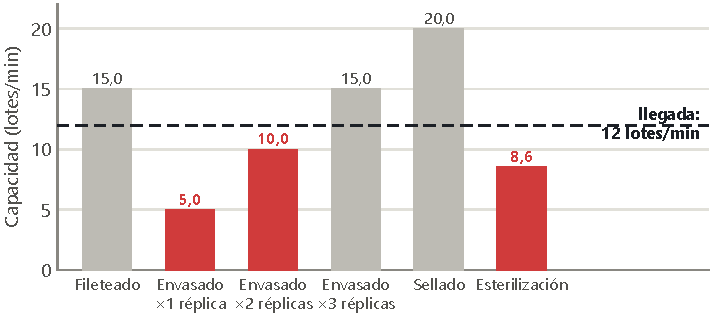
\includegraphics[width=0.86\textwidth]{figuras/fig_capacidad.pdf}
\caption{Capacidad de cada etapa (lotes/min) frente al ritmo de llegada del
protocolo. Las etapas bajo la línea segmentada no alcanzan a drenar lo que
les llega: ahí se forman las filas.}
\label{fig:capacidad}
\end{figure}

\subsection{Experimentos 1--3: el cuello se desplaza al escalar}

\begin{table}[H]
\centering
\caption{Resultado central: espera promedio por etapa (s) según réplicas de envasado.}
\label{tab:central}
\small
\begin{tabular}{C{2.2cm} C{2.2cm} C{2.2cm} C{2.2cm} C{2.6cm} C{2.4cm}}
\toprule
\textbf{Réplicas} & \textbf{Fileteado} & \textbf{Envasado} & \textbf{Sellado} & \textbf{Esterilización} & \textbf{Lead time} \\
\midrule
1 & 0{,}66 & \textbf{67{,}78 (crítico)} & 0{,}68 & 0{,}88 & 82{,}9 s \\
2 & 0{,}18 & 17{,}52 & 0{,}74 & \textbf{25{,}21 (crítico)} & 65{,}6 s \\
3 & 0{,}22 & 0{,}73 & 0{,}89 & \textbf{34{,}50 (crítico)} & 62{,}0 s \\
\bottomrule
\end{tabular}
\end{table}

\begin{itemize}[leftmargin=*]
  \item \textbf{1 réplica:} envasado acumula 14 lotes en cola y espera de
        67{,}8~s; el resto de la línea, ociosa a ratos, espera $<1$~s.
  \item \textbf{2 réplicas:} el reparto por demanda divide el trabajo (13/12
        lotes por réplica) y el tiempo efectivo de envasado baja a $\sim$6~s
        por lote. El cuello \textbf{se desplaza a esterilización} — la premisa
        del caso, demostrada con datos. Lead time: $-21$~\%.
  \item \textbf{3 réplicas:} envasado queda con capacidad sobrada (espera
        0{,}7~s), pero el lead time solo mejora otro 5~\%: el límite ya no
        está ahí. La inversión correcta siguiente sería una segunda autoclave,
        no una tercera envasadora.
\end{itemize}

\begin{figure}[H]
\centering
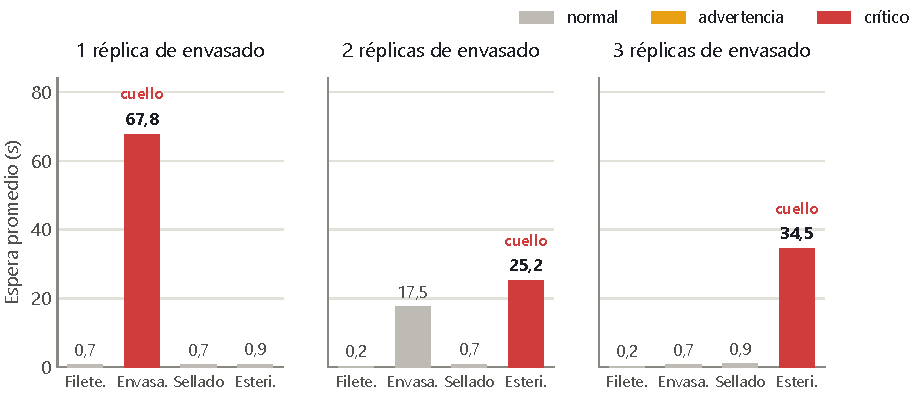
\includegraphics[width=0.98\textwidth]{figuras/fig_espera_replicas.pdf}
\caption{El resultado central, visto de una vez: la espera promedio por etapa
según el número de réplicas de envasado. El cuello (barra roja) no desaparece
al escalar: se desplaza de envasado a esterilización.}
\label{fig:espera_replicas}
\end{figure}

\begin{figure}[H]
\centering
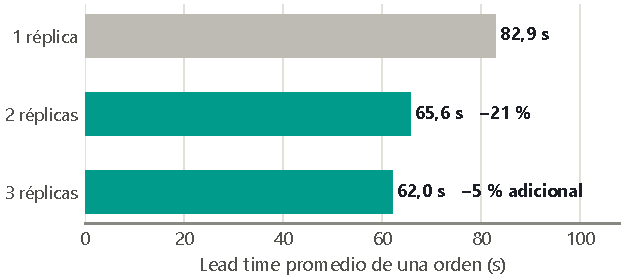
\includegraphics[width=0.7\textwidth]{figuras/fig_leadtime.pdf}
\caption{Lead time promedio de una orden (creación $\to$ terminada). La
segunda réplica compra un 21~\%; la tercera casi nada, porque el límite ya no
está en envasado.}
\label{fig:leadtime}
\end{figure}

Los tiempos de servicio medidos (4{,}6--5{,}0 / 12{,}2--13{,}0 / 3{,}3--3{,}5 /
7{,}3~s) coinciden con los ciclos configurados (4/12/3/7~s), lo que valida la
instrumentación.

\subsection{Experimento 4: balanceo dinámico con una réplica lenta}
\label{sec:exp4}

Dos réplicas normales más una configurada al doble de ciclo, sobre la misma
cola, 30 lotes: la lenta procesó \textbf{7} contra \textbf{11 y 12} de las
normales (Figura \ref{fig:replica_lenta}). Un round-robin habría repartido
10/10/10 sin importar la velocidad. Nadie asignó ese reparto: emergió de que
cada réplica reclama trabajo solo al quedar libre.

\begin{figure}[H]
\centering
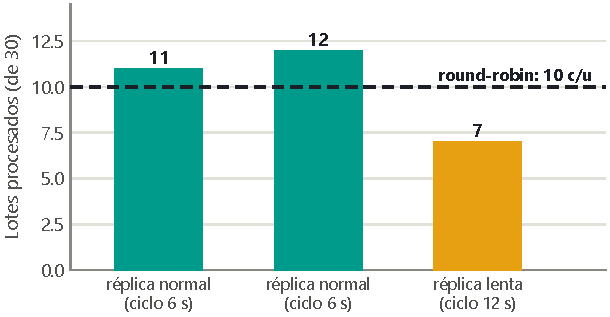
\includegraphics[width=0.62\textwidth]{figuras/fig_replica_lenta.pdf}
\caption{Balanceo dinámico con una réplica al doble de ciclo: el reparto se
adapta solo a la capacidad real de cada una, sin configuración ni
coordinación explícita.}
\label{fig:replica_lenta}
\end{figure}

\subsection{Experimento 5: saturación y recuperación automática}

Ráfaga de 25 órdenes de golpe (envasado $\times$2), observando
\texttt{/metricas/cuello} cada 15~s: a los 17~s la primera etapa pasa a
\texttt{advertencia} y a los 32~s a \texttt{crítico} — \textbf{sola}. La
Figura \ref{fig:saturacion} muestra la película completa: la congestión
recorre la línea como una ola (fileteado $\to$ envasado $\to$ esterilización)
y a los \textbf{278~s} las cuatro etapas están de vuelta en \texttt{normal}
\textbf{sin intervención alguna}: las esperas viejas salieron de la ventana
móvil. Detalle en \texttt{experimentos/resultados/exp5-saturacion.txt}.

\begin{figure}[H]
\centering
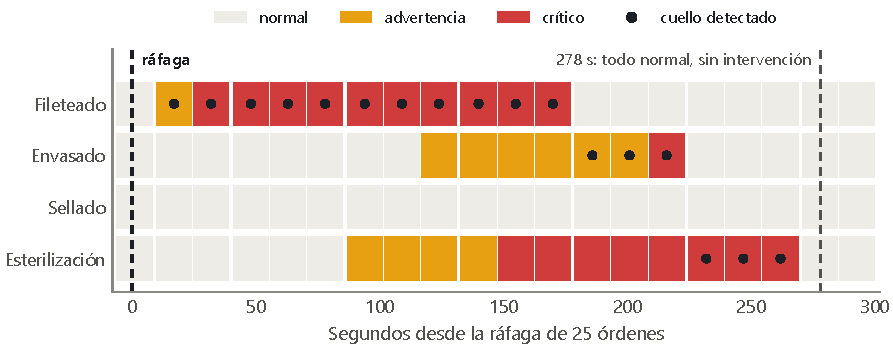
\includegraphics[width=0.98\textwidth]{figuras/fig_saturacion.pdf}
\caption{Experimento 5 como línea de tiempo de estados: cada fila es una
etapa y cada celda una sonda de \texttt{/metricas/cuello}. La congestión
avanza por la línea y el sistema vuelve a normal por sí solo.}
\label{fig:saturacion}
\end{figure}

La ráfaga deja además una lección de operación: con todo inyectado a la vez, el
cuello detectado inicialmente es la \emph{primera} etapa (ahí se apila la
cola), no la de mayor ciclo. El cuello depende del patrón de llegada, no solo
de los tiempos de proceso — por eso el protocolo de los experimentos 1--3
inyecta a ritmo constante.

% =============================================================================
\section{Manejo de errores}

Códigos verificados contra el sistema corriendo: \texttt{201} (creación),
\texttt{422} (cantidad $\leq 0$, producto vacío, filtro inválido — nunca 500),
\texttt{404} (orden inexistente), \texttt{503} (dependencia caída, con mensaje
en castellano). La UI nunca muestra un traceback: ante cualquier falla consulta
la salud de los tres servicios y \textbf{nombra al que realmente falta} — si
Redis cae, los demás siguen vivos y culpar al que responde lento enviaría a
buscar el error al lugar equivocado.

El hallazgo técnico de esta parte: con Redis detenido, los timeouts de socket
del cliente \textbf{no bastan}, porque el cuelgue ocurre antes, en la
resolución DNS (Docker elimina el nombre del contenedor detenido y
\texttt{getaddrinfo} tarda $\sim$45~s en rendirse — medido). La solución fue un
\textbf{plazo duro}: la consulta a Redis corre en un hilo aparte y se espera su
resultado a lo más 2~s; si no llega, se responde \texttt{503} de inmediato.
Resultado medido: \texttt{POST /ordenes} con Redis caído pasó de colgarse 46~s
a responder \texttt{503} en \textbf{2{,}1~s}, y \texttt{/metricas} responde
\texttt{200} en 2{,}0~s con \texttt{en\_cola: null} (un \texttt{null} honesto;
un 0 sería mentira).

Todos los servicios exponen \texttt{GET /salud} y tienen \texttt{healthcheck}
en el compose. El healthcheck mide \emph{vida}, no dependencias: un servicio
que responde 503 explicándose está sano — marcar \texttt{unhealthy} servicios
vivos habría provocado reinicios en cascada de contenedores que no tienen nada
malo.

% =============================================================================
\section{Reproducibilidad y despliegue}

\begin{lstlisting}
git clone <repositorio> && cd <carpeta>
docker compose up -d --build
# tablero en http://localhost:8501
\end{lstlisting}

Sin pasos manuales, sin instalar nada más que Docker \cite{docker}. La prueba se ejecutó
de verdad: clon en carpeta vacía $\to$ 8/8 contenedores \texttt{healthy} $\to$
orden creada por API recorre las cuatro etapas hasta \texttt{terminada} $\to$
tablero arriba. Toda la configuración tiene defaults funcionales
(\texttt{.env.example} documenta cada variable; no es obligatorio crearlo).
El README cubre instalación, uso, configuración, experimentos y diagnóstico de
fallas comunes.

% =============================================================================
\section{Resiliencia: cómo se abordaría}
\label{sec:resiliencia}

El enunciado no exige tolerancia a fallos y este proyecto, deliberadamente,
\textbf{detecta y explica} las fallas en vez de enmascararlas (sin reintentos,
sin circuit breaker). Si se necesitara operar esto en producción, la
arquitectura ya deja los puntos de corte correctos:

\begin{itemize}[leftmargin=*]
  \item \textbf{Estaciones (nodo B):} ya son resilientes en lo esencial — sin
        estado propio, reconectan solas (bucle de reintento del worker) y
        pueden multiplicarse o morir sin corromper nada. Lo único pendiente
        sería re-encolar el lote en curso si una réplica muere a mitad de
        ciclo (hoy ese lote se pierde de la cola; el patrón estándar es
        \texttt{BLMOVE} a una cola ``en proceso'' por réplica, devuelta a la
        cola principal por un barrendero al detectar un latido vencido).
  \item \textbf{Redis (nodo C):} es el punto único de falla del reparto. El
        camino estándar es Redis Sentinel (réplica + failover automático) o un
        broker con confirmaciones (el bonus Kafka apuntaba ahí): con
        \emph{acks}, un mensaje no confirmado vuelve a entregarse solo.
  \item \textbf{SQLite (nodo C):} suficiente para un nodo; con más escritores
        o failover se migraría a MySQL/PostgreSQL gestionado, cambiando solo
        el módulo \texttt{bd.py} de cada servicio.
  \item \textbf{APIs y UI (nodo A):} sin estado; con dos instancias y un
        balanceador HTTP delante quedarían en alta disponibilidad. Los
        healthchecks ya existentes son el insumo de ese balanceador.
\end{itemize}

La división en nodos de §\ref{sec:nodos} es exactamente la que hace estos
upgrades locales: cada mejora toca un nodo sin rediseñar los demás.

% =============================================================================
\section{Análisis crítico de dificultades}
\label{sec:dificultades}

\begin{enumerate}[leftmargin=*]
  \item \textbf{El entorno costó más que el primer código.} La virtualización
        venía deshabilitada en BIOS (\texttt{SVM Mode}); \texttt{wsl --install}
        no instaló ninguna distribución (hubo que pedir Ubuntu aparte); y
        Docker Desktop caía en cascada por sockets huérfanos de un arranque
        fallido que Windows no podía borrar, sembrando cada caída el bloqueo
        de la siguiente. Lección: el ``hola mundo'' de infraestructura es
        parte del proyecto y hay que presupuestarlo.
  \item \textbf{La condición de carrera hubo que fabricarla para verla.} Con
        el reclamo ingenuo, la ventana entre mirar y sacar es de
        microsegundos: sin duplicados no hay demostración. Se ensanchó con una
        espera artificial configurable (\texttt{DEMORA\_INGENUA}) hasta
        reproducir duplicados de forma confiable, y ambas versiones quedaron
        commiteadas — entender el problema antes de resolverlo.
  \item \textbf{``Le puse timeout'' no es verificable hasta medir el camino
        completo de la falla.} El cuelgue con Redis caído no estaba en el
        socket sino en el DNS (46~s medidos), que el timeout configurado no
        cubría. Hubo que aislar la falla por capas (resolución $\to$ conexión
        $\to$ lectura) y acotar la operación completa con un plazo duro.
  \item \textbf{Al acelerar una simulación se puede medir otra cosa.} El
        experimento de la réplica lenta con ciclos de $\sim$1~s dio un reparto
        casi parejo (21/20/19): a ese ritmo, el costo por lote lo dominaba la
        escritura de eventos en SQLite (seis procesos compitiendo por el lock
        sobre el volumen), no el ciclo simulado. Con ciclos de 6/12~s el
        overhead se vuelve despreciable y el resultado es el esperado
        (11/12/7). El overhead constante no escala con la simulación.
  \item \textbf{El cuello de botella depende del patrón de llegada.} Inyectar
        lotes de golpe apila todo en la primera cola y el sistema señala
        —correctamente— a fileteado. Entender que eso no era un bug sino una
        propiedad de las colas cambió el protocolo experimental y el guion de
        la demo: ritmo constante para responder ``¿qué etapa limita la
        producción?''.
\end{enumerate}

% =============================================================================
\section{Supuestos declarados}
\label{sec:supuestos}

\begin{enumerate}[leftmargin=*]
  \item Los tiempos de ciclo (4/12/3/7~s) son inventados, elegidos para que el
        desplazamiento del cuello sea demostrable en una demo corta. No
        representan una planta real; el escenario es ficticio.
  \item ``Procesar un lote'' se simula esperando el tiempo de ciclo; no hay
        trabajo real.
  \item Un lote representa una cantidad de latas del mismo formato; no se
        modelan latas individuales.
  \item El enunciado no fija qué persistir: decidimos órdenes y eventos, con
        las métricas siempre derivadas.
  \item El enunciado no define el criterio de cuello de botella ni umbrales:
        el criterio de §\ref{sec:criterio} es decisión nuestra.
\end{enumerate}

% =============================================================================
\section{Conclusiones}

El sistema cumple los requisitos del caso de punta a punta y sus afirmaciones
están respaldadas por mediciones reproducibles: el reparto por demanda
balancea sin conocer las réplicas (11/12/7 con una réplica lenta), la
extracción atómica elimina la condición de carrera (0 duplicados en 200
órdenes, contra duplicados reproducibles de la versión ingenua), el criterio de
espera en ventana móvil detecta el cuello de botella correcto incluso cuando no
es la etapa más lenta, y se recupera solo al bajar la carga. El resultado
central — el cuello se desplaza de envasado a esterilización al escalar de 1 a
2 réplicas, y una tercera ya no compra casi nada — es la demostración empírica
de que en una línea en serie \emph{el cuello de botella no se elimina: se
muda} \cite{goldratt}, y de que medir espera (no servicio) es lo que permite
verlo en vivo.

% =============================================================================
\begin{thebibliography}{9}

\bibitem{tanenbaum} M.~van Steen y A.~S. Tanenbaum, \emph{Distributed
Systems}, 4.ª ed. Maarten van Steen, 2023. Disponible en
\url{https://www.distributed-systems.net}.

\bibitem{kleppmann} M.~Kleppmann, \emph{Designing Data-Intensive
Applications}. Sebastopol, CA: O'Reilly Media, 2017.

\bibitem{goldratt} E.~M. Goldratt y J.~Cox, \emph{La Meta: un proceso de
mejora continua}, 3.ª ed. Great Barrington, MA: North River Press, 2004.

\bibitem{little} J.~D.~C. Little, ``A proof for the queuing formula
$L = \lambda W$'', \emph{Operations Research}, vol.~9, n.º~3, pp.~383--387,
1961.

\bibitem{redis} Redis Ltd., ``BRPOP — Redis command reference'',
documentación oficial de Redis 7, 2024. Disponible en
\url{https://redis.io/docs/latest/commands/brpop/}.

\bibitem{sqlite} SQLite Consortium, ``Write-Ahead Logging'', documentación
oficial de SQLite, 2024. Disponible en \url{https://www.sqlite.org/wal.html}.

\bibitem{docker} Docker Inc., ``Docker Compose overview'', documentación
oficial de Docker, 2024. Disponible en
\url{https://docs.docker.com/compose/}.

\end{thebibliography}

% =============================================================================
\appendix
\newpage

% =============================================================================
\section{Contratos completos de las APIs}
\label{anexo:apis}

Los tres servicios hablan REST sobre JSON. Todos exponen
\texttt{GET /salud}~$\rightarrow$~\texttt{200 \{"estado": "ok"\}}, que es lo que
consultan los \emph{healthchecks} de Docker Compose. El healthcheck mide
\textbf{vida del proceso}, no disponibilidad de sus dependencias: un servicio que
responde \texttt{503} explicando que Redis no está sigue estando sano.

\subsection{orders-api (puerto 8000)}

\subsubsection*{\texttt{POST /ordenes} — crear una orden de producción}

\begin{lstlisting}
Entrada:   { "producto": "jurel-425g", "cantidad": 10 }

Respuesta 201:
{
  "id": 1,
  "producto": "jurel-425g",
  "cantidad": 10,
  "estado": "en_proceso",
  "creada_en": "2026-08-21T17:30:00+00:00",
  "terminada_en": null
}
\end{lstlisting}

\begin{table}[H]
\centering
\footnotesize
\begin{tabular}{@{}lp{9.6cm}@{}}
\toprule
\textbf{Campo} & \textbf{Regla de validación} \\
\midrule
\texttt{producto} & string no vacío (tampoco solo espacios) \\
\texttt{cantidad} & entero \textbf{mayor que 0} — latas del lote \\
\bottomrule
\end{tabular}
\end{table}

Devuelve \textbf{422} si la entrada no cumple las reglas: nunca \texttt{500} y
nunca \texttt{201} con datos inválidos. Como efecto colateral, el \texttt{id} se
encola en \texttt{cola:fileteado} (Redis).

\subsubsection*{\texttt{GET /ordenes/\{id\}} y \texttt{GET /ordenes?estado=...}}

\begin{itemize}[leftmargin=*, itemsep=1pt]
  \item \texttt{GET /ordenes/\{id\}} $\rightarrow$ \textbf{200} con la orden
        completa, incluido \texttt{terminada\_en} (\texttt{null} si sigue en
        proceso). \textbf{404} si el id no existe.
  \item \texttt{GET /ordenes?estado=<en\_proceso|terminada>} $\rightarrow$
        \textbf{200} con la lista, filtrada si viene el parámetro.
        \textbf{422} si \texttt{estado} trae un valor fuera del catálogo.
\end{itemize}

\subsection{estacion (una imagen, cuatro despliegues)}

Toda la configuración entra por variables de entorno; \textbf{ningún} valor de
etapa está escrito en el código:

\begin{lstlisting}
NOMBRE_ETAPA=envasado
COLA_ENTRADA=cola:envasado
COLA_SALIDA=cola:sellado
TIEMPO_CICLO=12
\end{lstlisting}

\subsubsection*{\texttt{GET /estado}}

\begin{lstlisting}
{
  "etapa": "envasado",
  "replica_id": "envasado-a1b2c3",
  "procesadas": 17,
  "ocupada": true,
  "en_cola": 4
}
\end{lstlisting}

\texttt{en\_cola} es el largo actual de la cola de entrada (\texttt{LLEN}).
\texttt{replica\_id} se genera al arrancar — nombre de etapa más sufijo único —
y aparece también en cada línea de log, que es lo que permite atribuir cada lote
procesado a una réplica concreta en el experimento 4.

\subsection{metrics-api (puerto 8001)}

\subsubsection*{\texttt{GET /metricas}}

Por etapa, calculado siempre desde la tabla \texttt{eventos}:

\begin{lstlisting}
{
  "ventana_s": 60,
  "etapas": {
    "envasado": {
      "espera_promedio_s": 8.2,
      "servicio_promedio_s": 12.1,
      "en_cola": 4,
      "procesadas": 17
    }
  },
  "lead_time_promedio_s": 31.4
}
\end{lstlisting}

\subsubsection*{\texttt{GET /metricas/cuello}}

\begin{lstlisting}
{
  "cuello": "esterilizacion",
  "estados": { "fileteado": "normal", "envasado": "normal",
               "sellado": "normal", "esterilizacion": "critico" },
  "razon": "espera promedio 14.3 s en la ventana de 60 s,
            sobre el umbral critico"
}
\end{lstlisting}

\texttt{cuello} es \texttt{null} cuando ninguna etapa supera su umbral de
advertencia. El campo \texttt{razon} viene del servicio, no de la interfaz: el
diagnóstico y su justificación salen del mismo lugar.

\subsubsection*{\texttt{GET /metricas/historico}}

Serie temporal muestreada para los gráficos de la interfaz — la rúbrica exige
histórico además de tiempo real:

\begin{lstlisting}
{ "puntos": [ { "timestamp": "...", "etapa": "envasado",
                "espera_promedio_s": 8.2, "en_cola": 4 } ] }
\end{lstlisting}

\subsection{Códigos HTTP en uso}

\begin{table}[H]
\centering
\footnotesize
\begin{tabular}{@{}llp{8.2cm}@{}}
\toprule
\textbf{Código} & \textbf{Cuándo} & \textbf{Verificado con} \\
\midrule
\texttt{201} & Orden creada & \texttt{POST /ordenes} con cuerpo válido \\
\texttt{422} & Entrada inválida & \texttt{cantidad} $\leq 0$, \texttt{producto} vacío, \texttt{estado} fuera de catálogo \\
\texttt{404} & Recurso inexistente & \texttt{GET /ordenes/99999} \\
\texttt{503} & Dependencia caída & \texttt{docker compose stop redis} y luego \texttt{POST /ordenes} \\
\bottomrule
\end{tabular}
\end{table}

% =============================================================================
\newpage
\section{Esquema de datos y momentos de escritura}
\label{anexo:datos}

Dos tablas, y nada más. Todo lo demás se \textbf{calcula} desde \texttt{eventos}:
el dato guardado dos veces es el dato que termina contradiciéndose.

\begin{lstlisting}[language=SQL]
CREATE TABLE ordenes (
    id           INTEGER PRIMARY KEY AUTOINCREMENT,
    producto     TEXT    NOT NULL,
    cantidad     INTEGER NOT NULL CHECK (cantidad > 0),
    estado       TEXT    NOT NULL DEFAULT 'en_proceso',
    creada_en    TEXT    NOT NULL,   -- ISO 8601 UTC
    terminada_en TEXT                -- NULL hasta terminar
);

CREATE TABLE eventos (
    id         INTEGER PRIMARY KEY AUTOINCREMENT,
    orden_id   INTEGER NOT NULL REFERENCES ordenes(id),
    etapa      TEXT    NOT NULL,   -- fileteado | envasado |
                                   -- sellado | esterilizacion
    replica_id TEXT    NOT NULL,   -- que replica exacta lo hizo
    tipo       TEXT    NOT NULL,   -- entra_cola | inicia | termina
    timestamp  TEXT    NOT NULL    -- ISO 8601 UTC
);
\end{lstlisting}

\begin{table}[H]
\centering
\footnotesize
\begin{tabular}{@{}p{4.4cm}p{5.4cm}l@{}}
\toprule
\textbf{Momento} & \textbf{Quién escribe} & \textbf{Evento} \\
\midrule
La orden entra a una cola & orders-api, o la estación anterior & \texttt{entra\_cola} \\
Una réplica la saca de la cola (\texttt{BRPOP}) & la réplica & \texttt{inicia} \\
La réplica termina su ciclo & la réplica & \texttt{termina} \\
\bottomrule
\end{tabular}
\end{table}

Una orden que recorre las cuatro etapas genera \textbf{12 eventos}, tres por
etapa. El último \texttt{termina} de esterilización además marca
\texttt{ordenes.estado = 'terminada'} y escribe \texttt{terminada\_en}.

Los estados de una orden son solo dos, y es deliberado: \texttt{en\_proceso}
desde su creación y \texttt{terminada} al salir de esterilización. «En qué etapa
va» \textbf{no} es un estado guardado — se deriva del último evento de esa orden.
Guardarlo sería mantener dos versiones de la misma verdad.

De aquí salen las tres métricas del informe:

\begin{itemize}[leftmargin=*, itemsep=1pt]
  \item \textbf{Espera} en una etapa: $t(\texttt{inicia}) - t(\texttt{entra\_cola})$.
  \item \textbf{Servicio} en una etapa: $t(\texttt{termina}) - t(\texttt{inicia})$.
  \item \textbf{Lead time} de la orden: $t(\texttt{terminada\_en}) - t(\texttt{creada\_en})$.
\end{itemize}

Ninguna de las tres se almacena. Que los servicios medidos coincidan con los
ciclos configurados (4,8 / 12,4 / 3,4 / 7,3 s contra 4 / 12 / 3 / 7) es lo que
valida la instrumentación contra sí misma.

% =============================================================================
\newpage
\section{Capturas del tablero y verificación de errores}
\label{anexo:capturas}

Las tres capturas se tomaron sobre el sistema corriendo con
\texttt{docker compose up -d -{}-scale envasado=2}, inyectando carga real por
\texttt{POST /ordenes}. El color marca \textbf{importancia}, no identidad: lo
normal es gris y verde, y el color fuerte queda reservado para advertencia y
crítico, siempre acompañado de ícono y texto.

\textbf{Una aclaración necesaria.} En estas capturas la etapa señalada como
cuello es \textbf{fileteado}, no esterilización como en los experimentos del
§\ref{sec:experimentos}. No es una contradicción, y vale la pena explicarlo
porque es la primera pregunta que aparece al mirarlas: aquí los lotes se
inyectaron \textbf{en ráfaga} para forzar los estados de advertencia y crítico
rápidamente, y con llegadas en ráfaga la fila más larga se forma en la primera
etapa de la línea, que es donde entran. El detector responde correctamente a lo
que está pasando. Los experimentos del cuerpo usan llegadas \textbf{espaciadas}
—una cada 5~s— que es el régimen en el que la pregunta del caso tiene sentido, y
ahí el cuello aparece donde la aritmética de capacidad predice.

\begin{figure}[H]
\centering
\IfFileExists{figuras/tablero-normal.png}
  {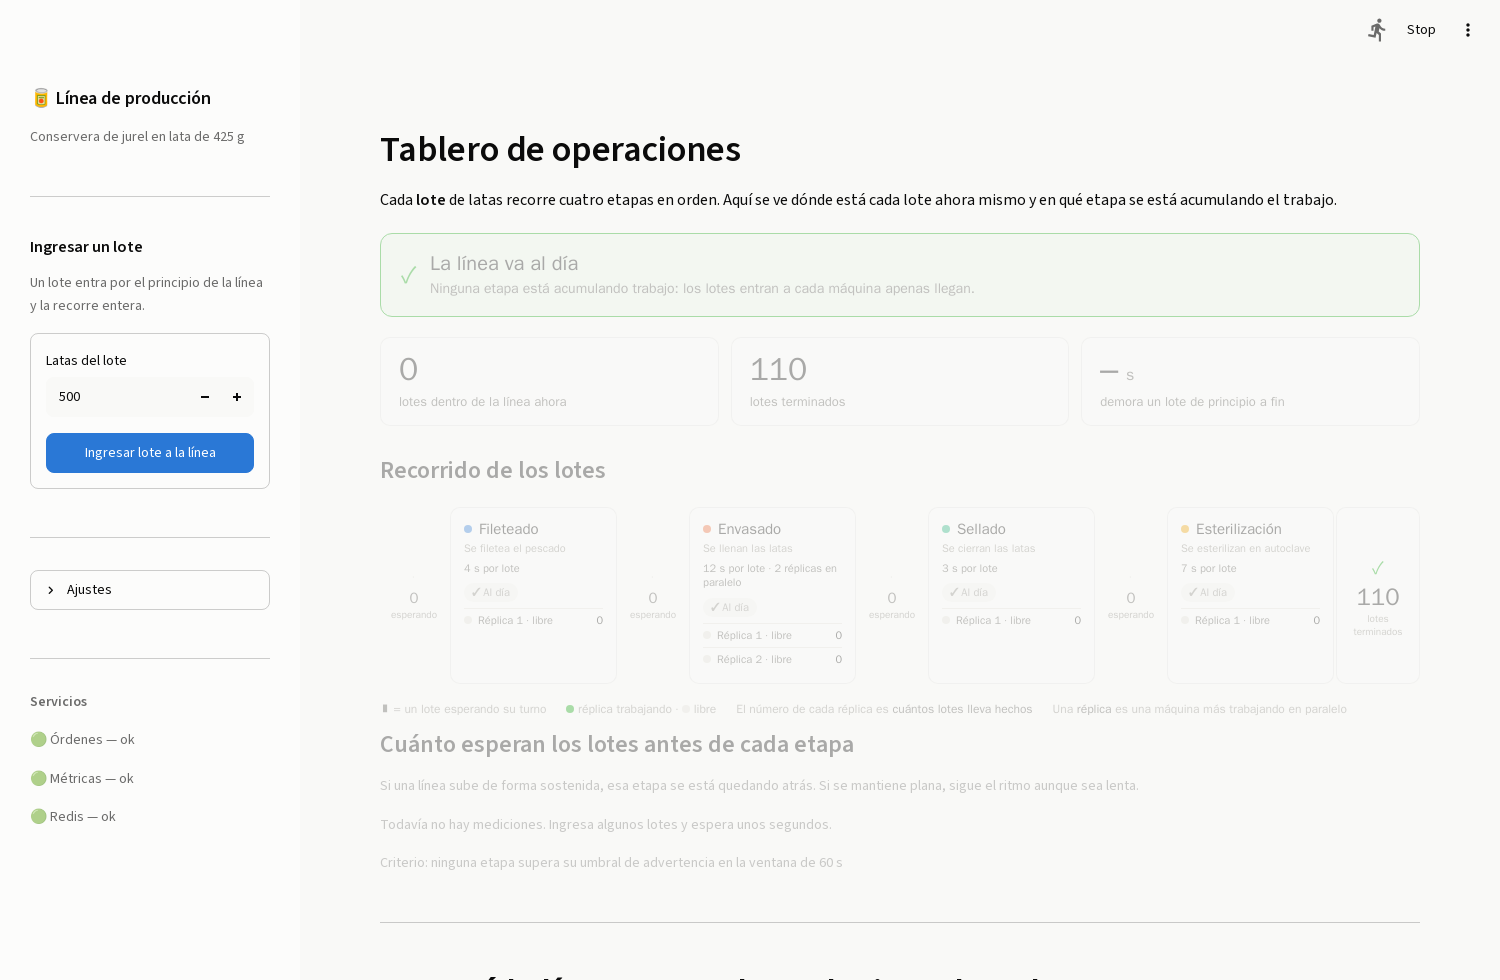
\includegraphics[width=0.96\textwidth]{figuras/tablero-normal.png}}
  {\fbox{\parbox{0.9\textwidth}{\centering\vspace{1cm}Captura pendiente:
   \texttt{figuras/tablero-normal.png}\vspace{1cm}}}}
\caption{Línea al día. Ninguna etapa supera su umbral de advertencia; el cartel
superior lo dice explícitamente y las cuatro etapas aparecen «Al día».}
\end{figure}

\begin{figure}[H]
\centering
\IfFileExists{figuras/tablero-advertencia.png}
  {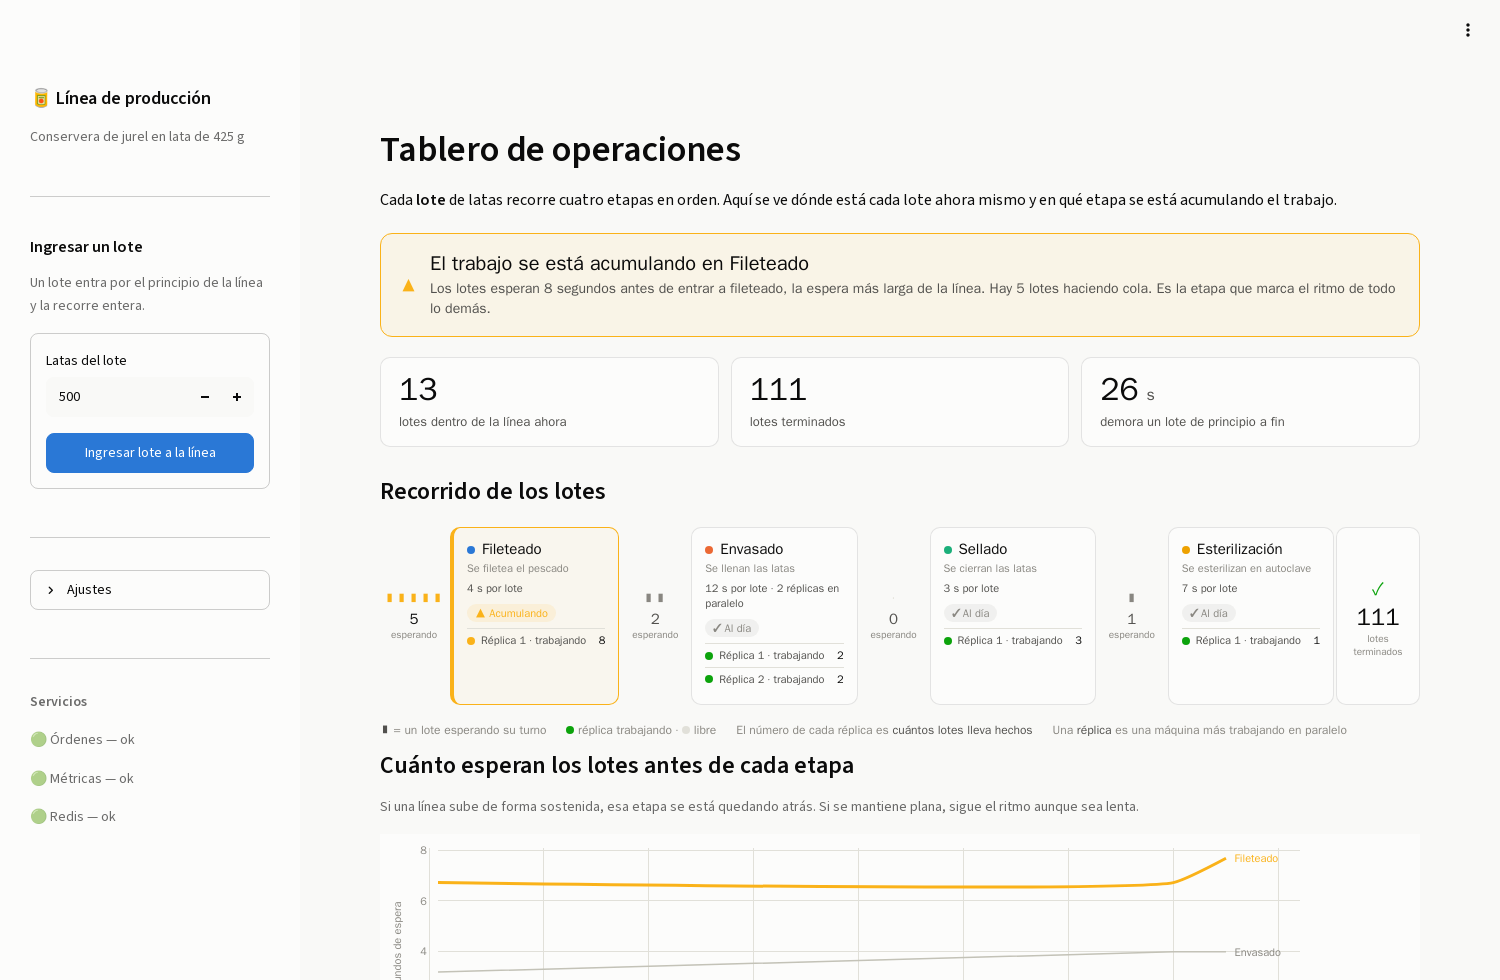
\includegraphics[width=0.96\textwidth]{figuras/tablero-advertencia.png}}
  {\fbox{\parbox{0.9\textwidth}{\centering\vspace{1cm}Captura pendiente:
   \texttt{figuras/tablero-advertencia.png}\vspace{1cm}}}}
\caption{Estado de \textbf{advertencia} tras inyectar 14 lotes espaciados 2~s.
La espera en fileteado llegó a 6,7~s contra su ciclo de 4~s: pasó el umbral de
advertencia ($1{,}5\times$) y no el crítico ($3\times$). El cartel nombra la
etapa, dice cuántos lotes hacen cola y da la cifra; la etapa aparece marcada
«Acumulando» y su curva de espera empieza a subir.}
\end{figure}

\begin{figure}[H]
\centering
\IfFileExists{figuras/tablero-critico.png}
  {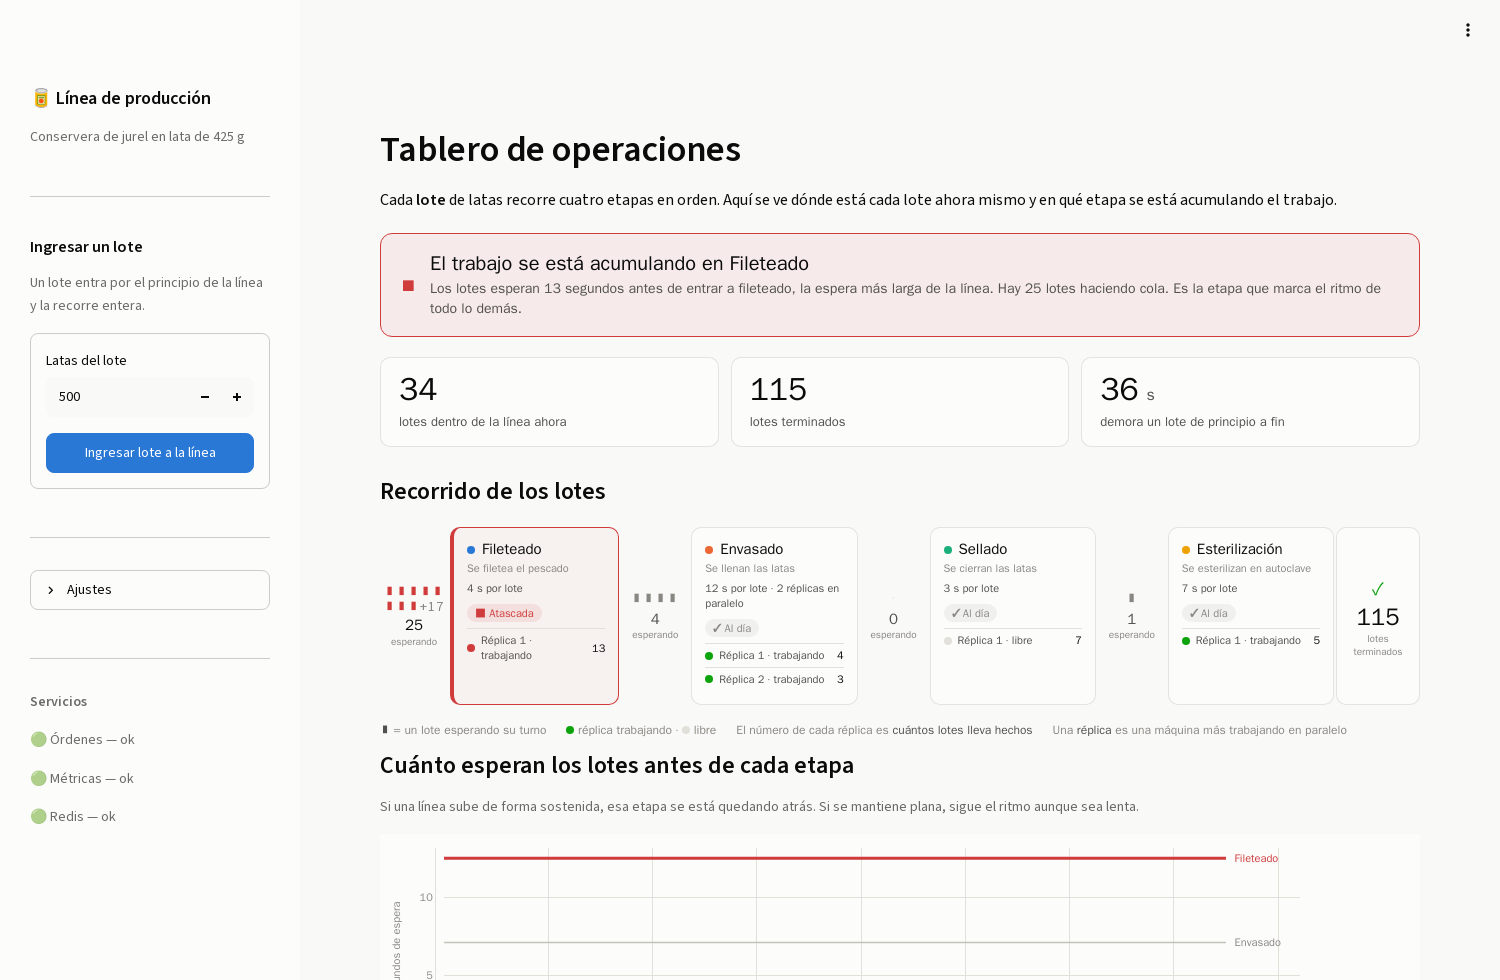
\includegraphics[width=0.96\textwidth]{figuras/tablero-critico.png}}
  {\fbox{\parbox{0.9\textwidth}{\centering\vspace{1cm}Captura pendiente:
   \texttt{figuras/tablero-critico.png}\vspace{1cm}}}}
\caption{Estado \textbf{crítico} tras una ráfaga de 25 lotes de golpe. La espera
en fileteado subió a 12,5~s contra su ciclo de 4~s, sobre el umbral crítico
($3\times$); la etapa queda marcada «Atascada» con 25 lotes en cola. El
diagnóstico y su razón vienen de \texttt{/metricas/cuello}, no de la interfaz:
el tablero solo lo muestra.}
\end{figure}

\subsection{Verificación de los códigos HTTP y de la caída de Redis}
\label{anexo:http}

El cuarto estado —Redis caído— se documenta con la traza medida contra el
sistema corriendo en vez de con una captura, porque es donde la evidencia
realmente está: los tiempos y los códigos son verificables y una imagen del
tablero no los muestra. La sesión completa, tal como salió:

\begin{lstlisting}
### CON REDIS ARRIBA
POST /ordenes            -> HTTP 201  en 0.013184s
GET  /salud (ordenes)    -> HTTP 200  en 0.003583s

### VALIDACION DE ENTRADA
POST cantidad=0          -> HTTP 422
POST producto vacio      -> HTTP 422
GET  /ordenes/99999      -> HTTP 404
GET  /ordenes?estado=xxx -> HTTP 422

### DETENIENDO REDIS   (docker compose stop redis)
POST /ordenes            -> HTTP 503  en 2.005218s
  {"detail":"sin conexion con el servicio de coordinacion (Redis);
             intente de nuevo"}
GET  /salud (ordenes)    -> HTTP 200  en 0.003470s
GET  /metricas/cuello    -> HTTP 200  en 2.011873s

### LEVANTANDO REDIS   (docker compose start redis)
POST /ordenes            -> HTTP 201  en 0.012831s
\end{lstlisting}

Tres cosas que esta traza prueba y que son el punto del §\ref{sec:resiliencia}:

\begin{enumerate}[leftmargin=*, itemsep=2pt]
  \item \textbf{El plazo duro funciona.} El \texttt{503} vuelve en
        \textbf{2,005~s}, no en los 46~s que medimos antes de descubrir que el
        cuelgue estaba en la resolución DNS y no en el socket. El
        \texttt{PLAZO\_REDIS\_S} configurado es 2~s y se cumple con cinco
        milésimas de margen.
  \item \textbf{El mensaje nombra al culpable real}, en castellano y sin
        \emph{traceback}: «sin conexión con el servicio de coordinación
        (Redis)». La interfaz muestra ese mismo texto, que viene del servicio.
  \item \textbf{El healthcheck sigue en 200 y en 3~ms.} El servicio de órdenes
        está \emph{vivo}: sabe que le falta una dependencia y lo dice. Si el
        healthcheck comprobara dependencias, Docker habría matado y reiniciado
        un contenedor que funcionaba perfectamente.
\end{enumerate}

Al volver a levantar Redis, la creación de órdenes responde \texttt{201} en 13~ms
sin reiniciar nada: la línea continúa donde quedó, porque las estaciones no
tienen estado propio y reconectan solas.

% =============================================================================
\newpage
\section{Salidas crudas de los experimentos}
\label{anexo:crudos}

Todo lo que sigue está versionado en \texttt{experimentos/resultados/} y se
reproduce con los guiones de \texttt{experimentos/}. Las figuras del cuerpo del
informe se generan desde estos mismos archivos con
\texttt{informe/figuras/generar\_figuras.py}: no hay ningún número transcrito a
mano entre la medición y el gráfico.

\subsection{Experimentos 1--3: el cuello se desplaza al escalar}

\begin{lstlisting}
--- exp1-envasado1-cuello.json ---
{"cuello":"envasado",
 "estados":{"fileteado":"normal","envasado":"critico",
            "sellado":"normal","esterilizacion":"normal"},
 "razon":"espera promedio 67.78 s en la ventana de 60 s,
          sobre el umbral critico (12 s de ciclo x 3)",
 "ventana_s":60.0}

--- exp2-envasado2-cuello.json ---
{"cuello":"esterilizacion",
 "estados":{"fileteado":"normal","envasado":"normal",
            "sellado":"normal","esterilizacion":"critico"},
 "razon":"espera promedio 25.21 s en la ventana de 60 s,
          sobre el umbral critico (7 s de ciclo x 3)",
 "ventana_s":60.0}

--- exp2-envasado2-metricas.json ---
{"ventana_s":60.0,"etapas":{
  "fileteado":     {"espera_promedio_s":0.18,"servicio_promedio_s":4.96,
                    "en_cola":0,"procesadas":31},
  "envasado":      {"espera_promedio_s":17.52,"servicio_promedio_s":12.58,
                    "en_cola":4,"procesadas":25},
  "sellado":       {"espera_promedio_s":0.74,"servicio_promedio_s":3.38,
                    "en_cola":0,"procesadas":24},
  "esterilizacion":{"espera_promedio_s":25.21,"servicio_promedio_s":7.25,
                    "en_cola":4,"procesadas":22}}}

--- exp3-envasado3-cuello.json ---
{"cuello":"esterilizacion",
 "estados":{"fileteado":"normal","envasado":"normal",
            "sellado":"normal","esterilizacion":"critico"},
 "razon":"espera promedio 34.5 s en la ventana de 60 s,
          sobre el umbral critico (7 s de ciclo x 3)",
 "ventana_s":60.0}

--- exp3-envasado3-metricas.json ---
{"ventana_s":60.0,"etapas":{
  "fileteado":     {"espera_promedio_s":0.22,"servicio_promedio_s":4.59,
                    "en_cola":0,"procesadas":31},
  "envasado":      {"espera_promedio_s":0.73,"servicio_promedio_s":12.24,
                    "en_cola":0,"procesadas":29},
  "sellado":       {"espera_promedio_s":0.89,"servicio_promedio_s":3.33,
                    "en_cola":0,"procesadas":28},
  "esterilizacion":{"espera_promedio_s":34.5,"servicio_promedio_s":7.3,
                    "en_cola":8,"procesadas":26}}}
\end{lstlisting}

\textbf{Limitación conocida.} El archivo
\texttt{exp1-envasado1-metricas.json} quedó \textbf{vacío} al capturarlo: la
consulta se hizo después de que la ventana móvil de 60~s ya se había vaciado.
El diagnóstico de cuello de ese experimento (\texttt{exp1-envasado1-cuello.json})
sí quedó guardado, y es de donde sale la cifra de 67,8~s de espera. Los valores
por etapa del experimento 1 en el cuerpo del informe provienen de esa corrida
registrada en la bitácora de la Fase 14, no de un archivo crudo. Se declara
aquí en vez de rehacerlo silenciosamente.

\subsection{Experimento 4: balanceo con una réplica lenta}

\begin{lstlisting}
--- exp4-replica-lenta.txt ---
envasado-88d690e0069d          11
envasado-b3573cf68ffd          12
envasado-lento-8550b032c252     7

ciclos: envasado=6s lento=12s, N=30 ordenes directas a cola:envasado
esperado round-robin: 10/10/10 - esperado por demanda: ~12/12/6
\end{lstlisting}

El reparto medido fue 11/12/7 contra el 10/10/10 que habría dado un
round-robin. La réplica lenta procesó un 40~\% menos que las rápidas sin que
nadie programara esa proporción: emergió de que cada réplica reclama un lote
solo cuando queda libre.

\subsection{Experimento 5: saturación y recuperación automática}

Ráfaga de 25 órdenes de golpe, sondeando \texttt{/metricas/cuello} cada 15~s.

\begin{lstlisting}
--- exp5-saturacion.txt (extracto) ---
t=1s    cuello=None       fileteado:normal       envasado:normal
t=17s   cuello=fileteado  fileteado:advertencia  envasado:normal
t=32s   cuello=fileteado  fileteado:critico      envasado:normal
t=48s   cuello=fileteado  fileteado:critico      envasado:normal
t=63s   cuello=fileteado  fileteado:critico      envasado:advertencia
...
t=278s  cuello=None       todas:normal
\end{lstlisting}

La congestión recorre la línea como una ola: aparece primero en fileteado, que
es donde entran los lotes, y se propaga aguas abajo. A los 278~s todo vuelve a
normal \textbf{sin intervención}, porque las esperas antiguas salieron de la
ventana móvil de 60~s. El sistema no «se arregla»: deja de estar congestionado y
la métrica lo refleja.

% =============================================================================
\newpage
\section{Historial de commits}
\label{anexo:commits}

El repositorio es
\url{https://github.com/CesarOlivares/Estructura-de-computadores-entrega-3}.
El trabajo está repartido entre los dos integrantes y distribuido en el tiempo,
no concentrado en una sesión final.

\begin{table}[H]
\centering
\footnotesize
\begin{tabular}{@{}lrl@{}}
\toprule
\textbf{Autor} & \textbf{Commits} & \textbf{Aporte principal} \\
\midrule
César Olivares & 27 & Servicios, Redis, persistencia, métricas, informe \\
Simón García-Huidobro & 15 & Tablero Streamlit, demo de la carrera, lanzadores, defensa \\
\midrule
\textbf{Total} & \textbf{42} & 21--25 de agosto de 2026 \\
\bottomrule
\end{tabular}
\end{table}

Los tres primeros commits son cargas por la interfaz web de GitHub, anteriores a
fijar la convención del equipo. Desde \texttt{chore: initialize repository} en
adelante se usa Conventional Commits, con un commit por fase verificada.

\begin{lstlisting}
7a9d44b 2026-08-21 Cesar   Add files via upload
b05cb63 2026-08-21 Cesar   Add files via upload
fba5747 2026-08-21 Cesar   Add files via upload
1f3b57c 2026-08-21 Cesar   chore: initialize repository
bb87555 2026-08-21 Cesar   demo: throwaway queue prototype
176a0b1 2026-08-21 Cesar   docs: close phase 0 environment log
4330ff4 2026-08-21 Cesar   docs: define api contracts and data model
8253914 2026-08-21 Cesar   feat: minimal orders api with validation
6398e77 2026-08-21 Cesar   feat: add redis queue and healthcheck
ec6c211 2026-08-21 Cesar   feat: station worker consuming orders
05efcc9 2026-08-21 Cesar   feat: reproduce race condition with naive claiming
3f1c79b 2026-08-21 Cesar   feat: implement atomic order claiming
c9c6fc3 2026-08-21 Cesar   test: verify no duplicate processing under load
d178cec 2026-08-21 Cesar   feat: scale stations and expose replica identity
e435d42 2026-08-21 Cesar   feat: dynamic load balancing with configurable times
1c8ce5a 2026-08-21 Cesar   feat: persist orders and events in sqlite
28db438 2026-08-21 Cesar   feat: metrics service with lead time breakdown
b77b6a1 2026-08-21 Cesar   feat: bottleneck detection with sliding window
c937045 2026-08-21 Simon   feat: streamlit operations dashboard
3e9abf0 2026-08-21 Simon   docs: readme with setup and run instructions
0b74b9b 2026-08-22 Simon   docs: align phase 11 log with team template
f3d8d74 2026-08-22 Cesar   feat: error handling and http status codes
44181d2 2026-08-22 Cesar   docs: env example and reproducibility notes
51858f2 2026-08-22 Cesar   docs: readme verified on clean clone
02bfe33 2026-08-22 Cesar   docs: experiment results for 1, 2 and 3 replicas
7182916 2026-08-22 Cesar   docs: architecture decisions and assumptions
abfb9bb 2026-08-23 Simon   fix: count processed orders per stage
1d0d90c 2026-08-23 Simon   refactor: extract claim strategies into shared module
5d4b125 2026-08-23 Simon   feat: race condition demo in the dashboard
4fbcd17 2026-08-23 Simon   feat: one-click launcher for windows, macos, linux
d99d7ac 2026-08-23 Simon   docs: phase 16 log, readme and defence guide
25e84cb 2026-08-23 Cesar   chore: tidy repo layout for delivery
e060912 2026-08-23 Cesar   docs: report with charts, diagrams and bibliography
08c47c3 2026-08-23 Cesar   docs: defense slides with charts, exported to pdf
ce6a19d 2026-08-23 Cesar   docs: demo slide covers the race comparison
7ed4fe4 2026-08-25 Simon   chore: move course material into enunciado/
9d1ae9f 2026-08-25 Simon   chore: drop the internal working plan
603c0a5 2026-08-25 Simon   docs: readme points to the deliverables
669762a 2026-08-25 Simon   docs: slides drop topic numbering, compile on Overleaf
fff994f 2026-08-25 Simon   docs: second format for the defence slides
86cc321 2026-08-25 Simon   fix: slides embed a font dvipdfmx can write
95b4894 2026-08-25 Simon   docs: both slide PDFs compiled and current
\end{lstlisting}

La condición de carrera está en el historial como dos commits consecutivos:
\texttt{05efcc9} la reproduce con el reclamo ingenuo y \texttt{3f1c79b} la
elimina con extracción atómica. No se resolvió el problema antes de tenerlo.

% =============================================================================
\newpage
\section{Bitácoras por fase}
\label{anexo:fases}

El proyecto se organizó en fases; cada una deja una bitácora en
\texttt{docs/fases/} escrita al cerrarla, con objetivo, qué se logró,
dificultades encontradas y pendientes. Son el insumo directo del análisis
crítico del §\ref{sec:dificultades} de este informe.

\begin{table}[H]
\centering
\footnotesize
\begin{tabular}{@{}lp{7.4cm}l@{}}
\toprule
\textbf{Archivo} & \textbf{Fase} & \textbf{Estado} \\
\midrule
\texttt{fase-0-entorno.md} & Entorno y repositorio & Cerrada 21/08 \\
\texttt{fase-2-diseno.md} & Diseño en papel & Diseño listo \\
\texttt{fase-3-orders-api.md} & \texttt{orders-api} mínima en Docker & Cerrada 21/08 \\
\texttt{fase-4-redis.md} & Redis y la cola & Cerrada 21/08 \\
\texttt{fase-5-estacion.md} & Una estación consume & Cerrada 21/08 \\
\texttt{fase-6-carrera.md} & Condición de carrera: provocarla y resolverla & Cerrada 21/08 \\
\texttt{fase-7-balanceo.md} & Balanceo dinámico con N réplicas & Cerrada 21/08 \\
\texttt{fase-8-persistencia.md} & Persistencia & Cerrada 21/08 \\
\texttt{fase-9-metricas.md} & Métricas & Cerrada 21/08 \\
\texttt{fase-10-cuello-de-botella.md} & Cuello de botella y estados & Cerrada 21/08 \\
\texttt{fase-11-ui.md} & Interfaz Streamlit & Cerrada 21/08 \\
\texttt{fase-12-errores.md} & Errores, logging y healthchecks & Cerrada 22/08 \\
\texttt{fase-13-reproducibilidad.md} & Reproducibilidad & Cerrada 22/08 \\
\texttt{fase-14-experimentos.md} & Experimentos & Cerrada 22/08 \\
\texttt{fase-15-informe.md} & Informe y defensa & En curso \\
\texttt{fase-16-demostracion-ui.md} & La demostración de la carrera en el tablero & Cerrada 23/08 \\
\bottomrule
\end{tabular}
\end{table}

La Fase 1 no tiene bitácora propia: fue el prototipo desechable de cola y
trabajadores que vive en \texttt{demo/} con su propio README, y su resultado
(reparto 5/5/5 con tres trabajadores iguales, sin duplicados) quedó registrado
ahí. La Fase 2 aparece como «diseño listo» y no «cerrada» a propósito: la prueba
de equipo que el plan exige para darla por terminada —ambos integrantes
respondiendo el cuestionario de \texttt{docs/diseno.md} §6 sin mirar el
documento— es la única condición de cierre que quedó pendiente.

\end{document}
